\documentclass[a4paper,10pt]{article}
\usepackage{graphicx}
\usepackage[left=1in,right=1in,top=1in,bottom=1in]{geometry}
\usepackage{hyperref}
\usepackage{fancyhdr}

\pagestyle{fancy}
\lhead{\textbf{Daniel Velarde Kubber}}
\rhead{\textbf{Currículum Vitae}}
\cfoot{\thepage}

\begin{document}

% Agrega tu fotografía en la esquina superior derecha
\begin{minipage}[t]{0.7\textwidth}
  % Tu contenido existente va aquí
\end{minipage}
\hfill
\begin{minipage}[t]{0.3\textwidth}
  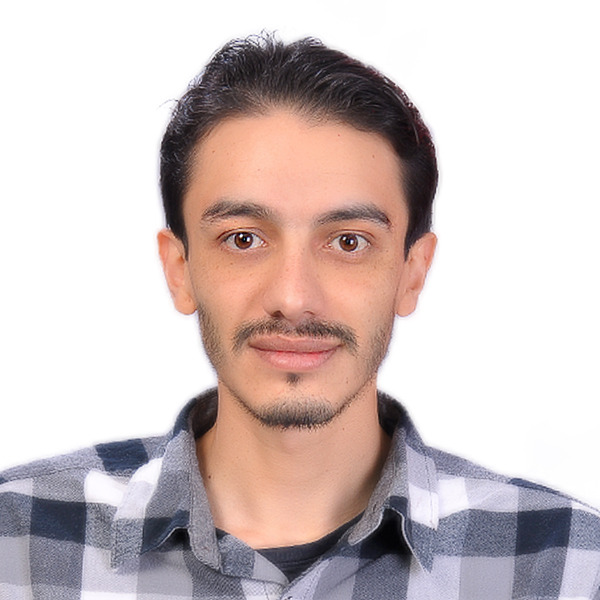
\includegraphics[width=2.5cm]{photocv.jpeg}
\end{minipage}

\begin{center}
\textbf{\LARGE Daniel Velarde Kubber}
\end{center}

\section*{Información de Contacto}
\begin{tabular}{ll}
    Dirección: & Cota Cota, Calle 37, Edificio Amelia 2, La Paz - Bolivia \\
    Teléfono: & +591 76778873 \\
    Fecha de Nacimiento: & 16 de enero de 1989 \\
    Correo Electrónico: & daniel.velarde.kubber@gmail.com \\
    LinkedIn: & \url{https://www.linkedin.com/in/daniel-velarde-kubber-027a8951/} \\
\end{tabular}

\section*{Resumen Profesional}
Apasionado por los datos y la tecnología, soy un profesional orientado a resultados con antecedentes en Ingeniería Industrial y de Sistemas. Desde mis primeros días como administrador de bases de datos hasta mi papel como empresario y CEO en Hobbie 3D Print, he perfeccionado mis habilidades en la gestión de datos, el liderazgo estratégico y la competencia técnica.

Mi trayectoria profesional, que incluye experiencia práctica en la programación de impresoras 3D, administración de bases de datos y gestión de proyectos, refleja mi dedicación a aprovechar los datos para impulsar el éxito empresarial. Me impulsa el poder de la innovación y prospero en el desafío de fomentar el crecimiento.

Con un fuerte compromiso con la toma de decisiones basadas en datos, estoy emocionado por aplicar mi experiencia en nuevas oportunidades y contribuir a los campos de ingeniería de datos, análisis de datos y ciencia de datos.

\section*{Educación}
\begin{tabular}{p{3cm}p{12cm}}
    2012 & Ingeniero Industrial y de Sistemas, Universidad Privada Boliviana, Cochabamba - Bolivia \\
\end{tabular}

\section*{Experiencia Profesional}

\textbf{Empresa:} Universidad Católica Boliviana (Docente Post Proceso de impresiones 3D)  
\textbf{Duración:} [sept 2023] - [oct 2023]

\textbf{Descripción de mis responsabilidades y logros:}
\begin{itemize}
    \item El curso buscó formar y capacitar profesionales en el correcto post proceso de una impresión 3D, otorgándoles herramientas y técnicas adecuadas para acabados profesionales en piezas mecánicas o estéticas. El contenido del curso se dividió en las siguientes unidades temáticas:
    \item Unidad 1: Suavizado de impresiones.
    \item Unidad 2: Aplicación de imprimación.
    \item Unidad 3: Aplicación de luces y sombras en primer.
    \item Unidad 4: Limpieza, cuidado y partes que componen el aerógrafo.
    \item Unidad 5: Capa base, técnicas de pincel y lavado en aceite.
    \item Unidad 6: Aplicación de luces en pincel seco y perfilad.

\end{itemize}
\vspace{15pt} % Ajusta el valor para controlar la cantidad de espacio
\textbf{Empresa:} Hobbie 3D Print (Propietario y CEO)  
\textbf{Duración:} [2018] - [2023]

\textbf{Descripción de mis responsabilidades y logros:}
\begin{itemize}
    \item Liderazgo Estratégico: Fui el líder en la dirección estratégica general de Hobbie 3D Print, guiando a la empresa desde su inicio durante cuatro años de crecimiento y éxito continuo.
    \item Competencia Técnica: Adquirí un profundo conocimiento de la programación de impresoras 3D, lo que permitió la optimización de los procesos de impresión y aseguró la entrega de productos impresos en 3D de alta calidad.
    \item Gestión Práctica: Administré todos los aspectos de la empresa, desde las operaciones diarias, la gestión de proyectos y el control de calidad hasta el servicio al cliente. Supervisé a un equipo de profesionales dedicados y garanticé la entrega oportuna de proyectos.
    \item Marketing y Branding: Formulé y ejecuté estrategias de marketing integrales que aumentaron la visibilidad de la marca y atrajeron una base sustancial de clientes. Logré un crecimiento significativo en los ingresos durante el período de cuatro años.
    \item Conocimiento Financiero: Demostré competencia en la gestión financiera, incluida la elaboración de presupuestos, la previsión y el control de costos, lo que resultó en rentabilidad constante y estabilidad financiera.
    \item Administración: Optimicé procesos administrativos, incluida la gestión de inventarios, el cumplimiento de pedidos y la logística de la cadena de suministro, lo que mejoró la eficiencia de la empresa y garantizó la satisfacción del cliente.
    \item Participación del Cliente: Cultivé y mantuve relaciones sólidas con los clientes, garantizando experiencias excepcionales y negocios repetidos, lo que resultó en una alta retención de clientes.
    \item Innovación y Desarrollo de Productos: Participé activamente en el diseño y desarrollo de modelos 3D, fomentando la innovación de productos y manteniéndome al tanto de las tendencias de la industria.
    \item Cumplimiento y Regulación: Garanticé el cumplimiento total con las normas y regulaciones de la industria, fomentando la confianza y la credibilidad dentro de la comunidad de impresión 3D.
    \item Crecimiento Empresarial: Logré un crecimiento significativo de la empresa, con un aumento anual de los ingresos.

\end{itemize}

\textbf{Empresa:} Velarde Construcciones SRL  
\textbf{Duración:} [2013] - [2018]

\textbf{Descripción de mis responsabilidades y logros:}
\begin{itemize}
    \item Crecimiento Profesional: Comencé como mensajero y gradualmente avancé a un papel con responsabilidades significativas durante seis años.
    \item Gestión de Proyectos: Lideré y ejecuté varios proyectos, demostrando sólidas habilidades de gestión de proyectos y asegurando una finalización oportuna.
    \item Transferencia Electrónica de Fondos: Gestioné transferencias electrónicas de fondos para la empresa, optimizando los procesos financieros.
    \item Operaciones de Importación/Exportación: Manejé con éxito operaciones internacionales de importación/exportación de bienes, asegurando el cumplimiento de las regulaciones pertinentes.
    \item Administración de Bases de Datos (MySQL): Supervisé la gestión de la base de datos MySQL, incluida la importación, exportación, copia de seguridad y resolución de problemas diarios, garantizando la integridad y disponibilidad de los datos.
    \item Gestión de Inventarios: Implementé sistemas eficientes de gestión de inventarios, mejorando el control y minimizando errores.
    \item Control de Inventarios: Mantuve un control preciso de los inventarios, reduciendo el desperdicio y ahorrando costos.
    \item Contabilidad: Contribuí a la salud financiera de la organización a través de prácticas contables meticulosas.
\end{itemize}

\textbf{Empresa:} Aceros Arequipa  
\textbf{Duración:} [2012] - [2013]

\textbf{Descripción de mis responsabilidades y logros:}
\begin{itemize}
    \item Comienzo Temprano en la Carrera: Inicié mi carrera profesional como Administrador de Bases de Datos en Aceros Arequipa, una oportunidad valiosa justo después de graduarme de la universidad.
    \item Administración de Bases de Datos (MySQL): Gestioné la base de datos MySQL, incluida la gestión de datos, la optimización y la seguridad.
    \item Máquinas Virtuales: Supervisé despliegues de máquinas virtuales, asegurando la utilización eficiente de los recursos.
    \item Soporte de TI: Brindé soporte integral al departamento de TI, resolviendo problemas técnicos y ayudando a los colegas con problemas relacionados con sus PC.
    \item Seguridad de Datos: Desempeñé un papel fundamental en la seguridad de la base de datos de la empresa y en la infraestructura de TI, garantizando la integridad y protección de los datos.
\end{itemize}

\section*{Licencias y Certificaciones}
\begin{description}
    \item[Certificado:] Introducción a la Ingeniería de Datos, Coursera, agosto de 2023
    \item[Identificación de Credencial:] 9S9DAUQLBP27
    \item[URL del Certificado:] \url{https://www.coursera.org/account/accomplishments/certificate/9S9DAUQLBP27}
\end{description}

\vspace{1pt} % Ajusta el valor para controlar la cantidad de espacio

\begin{description}
    \item[Certificado:] Introducción a las Bases de Datos Relacionales (RDBMS), Coursera, agosto de 2023
    \item[Identificación de Credencial:] SG8MV2SLJXHC
    \item[URL del Certificado:] \url{https://www.coursera.org/account/accomplishments/certificate/SG8MV2SLJXHC}
\end{description}

\vspace{1pt} % Ajusta el valor para controlar la cantidad de espacio

\begin{description}
    \item[Certificado:] Python para Ciencia de Datos, Inteligencia Artificial y Desarrollo, Coursera, agosto de 2023
    \item[Identificación de Credencial:] X6P3RHPT255M
    \item[URL del Certificado:] \url{https://www.coursera.org/account/accomplishments/certificate/X6P3RHPT255M}
\end{description}

\vspace{1pt} % Ajusta el valor para controlar la cantidad de espacio

\begin{description}
    \item[Certificado:] Proyecto Python para Ingeniería de Datos, Coursera, agosto de 2023
    \item[Identificación de Credencial:] WEQ4BMAGTZZN
    \url{https://www.coursera.org/account/accomplishments/certificate/WEQ4BMAGTZZN}
\end{description}

\vspace{1pt} % Ajusta el valor para controlar la cantidad de espacio

\begin{description}
    \item[Certificado:] Introducción Práctica a los Comandos de Linux y Scripting de Shell, Coursera, septiembre de 2023
    \item[Identificación de Credencial:] TN4F6WG8DWKB
    \item[URL del Certificado:] \url{https://www.coursera.org/account/accomplishments/certificate/TN4F6WG8DWKB}
\end{description}

\vspace{1pt} % Ajusta el valor para controlar la cantidad de espacio

\begin{description}
    \item[Certificado:] Bases de Datos y SQL para Ciencia de Datos con Python, Coursera, septiembre de 2023
    \item[Identificación de Credencial:] AZMNGATPHMYT
    \item[URL del Certificado:] \url{https://www.coursera.org/account/accomplishments/certificate/AZMNGATPHMYT}
\end{description}

\vspace{1pt} % Ajusta el valor para controlar la cantidad de espacio

\begin{description}
    \item[Certificado:] Administración de Bases de Datos Relacionales (DBA), Coursera, septiembre de 2023
    \item[Identificación de Credencial:] EASM4DYAZY4L
    \item[URL del Certificado:] \url{https://www.coursera.org/account/accomplishments/certificate/EASM4DYAZY4L}
\end{description}

\vspace{1pt} % Ajusta el valor para controlar la cantidad de espacio

\begin{description}
    \item[Certificado:] ETL y Canalización de Datos con Shell, Airflow y Kafka, Coursera, septiembre de 2023
    \item[Identificación de Credencial:] HGASHU2DN99L
    \item[URL del Certificado:] \url{https://www.coursera.org/account/accomplishments/certificate/HGASHU2DN99L}
\end{description}
\vspace{1pt} % Adjust the value to control the amount of space

\begin{description}
    \item[Certificate:] IBM Data Engineering Specialization, Coursera, October 2023
    \item[Certificate URL:] \url{https://www.coursera.org/account/accomplishments/specialization/W8KEPFZX9XGF}
\end{description}
\vspace{1pt} % Adjust the value to control the amount of space
\begin{description}
    \item[GitHub:] \url{https://github.com/DanielVelarde/briefcase.git}
\end{description}

\section*{Habilidades}
\begin{tabular}{p{4.5cm}p{4.5cm}p{4.5cm}}
    Bases de Datos & Arquitectura de Datos & Transferencia Electrónica de Fondos \\
    Seguridad de Bases de Datos & Diseño de Bases de Datos & Operaciones de Importación/Exportación \\
    Administración de Bases de Datos & RDBMS & Gestión de Inventarios \\
    Servidores de Bases de Datos & Canalización de Datos & Control de Inventarios \\
    SQL & Visualización de Datos & Contabilidad Básica \\
    IBM Db2 & Bokeh & Gestión de Proyectos \\
    MySQL & Matplotlib & Marketing Digital \\
    NoSQL & Pandas & Microsoft Office \\
    ETL (Extract, Load, Transform) & NumPy & Modelado 3D \\
    Jupyter Notebook & IBM Cloud & Impresión 3D \\
    Python & Linux & Desarrollo de Productos \\
    C++ & C\# & \\
    PostgreSQL & & \\
\end{tabular}

\section*{Idiomas}
\begin{itemize}
    \item Español: Proficiencia Nativa
    \item Inglés: Competente
    % Agrega más idiomas según corresponda
\end{itemize}

\section*{Intereses}
En mi tiempo libre, tengo pasión por la lectura de libros de fantasía, sumergiéndome en mundos épicos que recuerdan a "El Señor de los Anillos" y "World of Warcraft". También disfruto de los videojuegos, tanto como forma de entretenimiento como para relacionarme con mis hijos.

Soy un aprendiz ávido y encuentro alegría en la programación, explorando varios lenguajes de programación y, en un momento, incursionando en el desarrollo de juegos con Unity. Además, tengo un lado creativo que expreso a través de la pintura de miniaturas, un pasatiempo que me permite combinar mi amor por el arte y la artesanía.


\section*{Referencias Personales}
\renewcommand{\refname}{}

\begin{thebibliography}{}
\bibitem{Universidad Católica Boliviana} Universidad Católica Boliviana
  \begin{description}
    \item[Nombre:] Ing. Fabio Richard Diaz Palacios
    \item[Teléfono:] +591 72082521
  \end{description}


\bibitem{hobbie3dprint} Hobbie 3D Print
  \begin{description}
    \item[Nombre:] Ing. Daniel Velarde Kubber
    \item[Email:] daniel.velarde.kubber@gmail.com
    \item[Teléfono:] +591 76778873
    \item[Facebook:] \url{https://www.facebook.com/Hobbie3DPrint/}
  \end{description}

\bibitem{velardeconstrucciones} Velarde Construcciones SRL
  \begin{description}
    \item[Nombre:] Ing. Carlos Estrada Roblin
    \item[Email:] cestradaroblin@gmail.com
    \item[Teléfono:] +591 77538902
  \end{description}

\bibitem{acerosarequipa} Aceros Arequipa
  \begin{description}
    \item[Nombre:] Ing. Daniel Fernando Balandra Mallma
    \item[Email:] daniel.balandra@repareq.com
    \item[Teléfono:] +591 77200296
  \end{description}

\end{thebibliography}
\end{document}


\end{document}

